\section{Model formulation}\label{formulation}

In this section, we describe the models that are used to develop our multi-resolution scheme.  We start by presenting the governing equations to model hydraulic fracture in poroelastic rock that forms the basis for the solver at the global scale.  We then describe a phase-field model for fracture that forms the basis for the solver used in local subdomains near the crack tips.

\subsection{Governing equations for hydraulic fracture}

\begin{figure}[h]
    \centering
    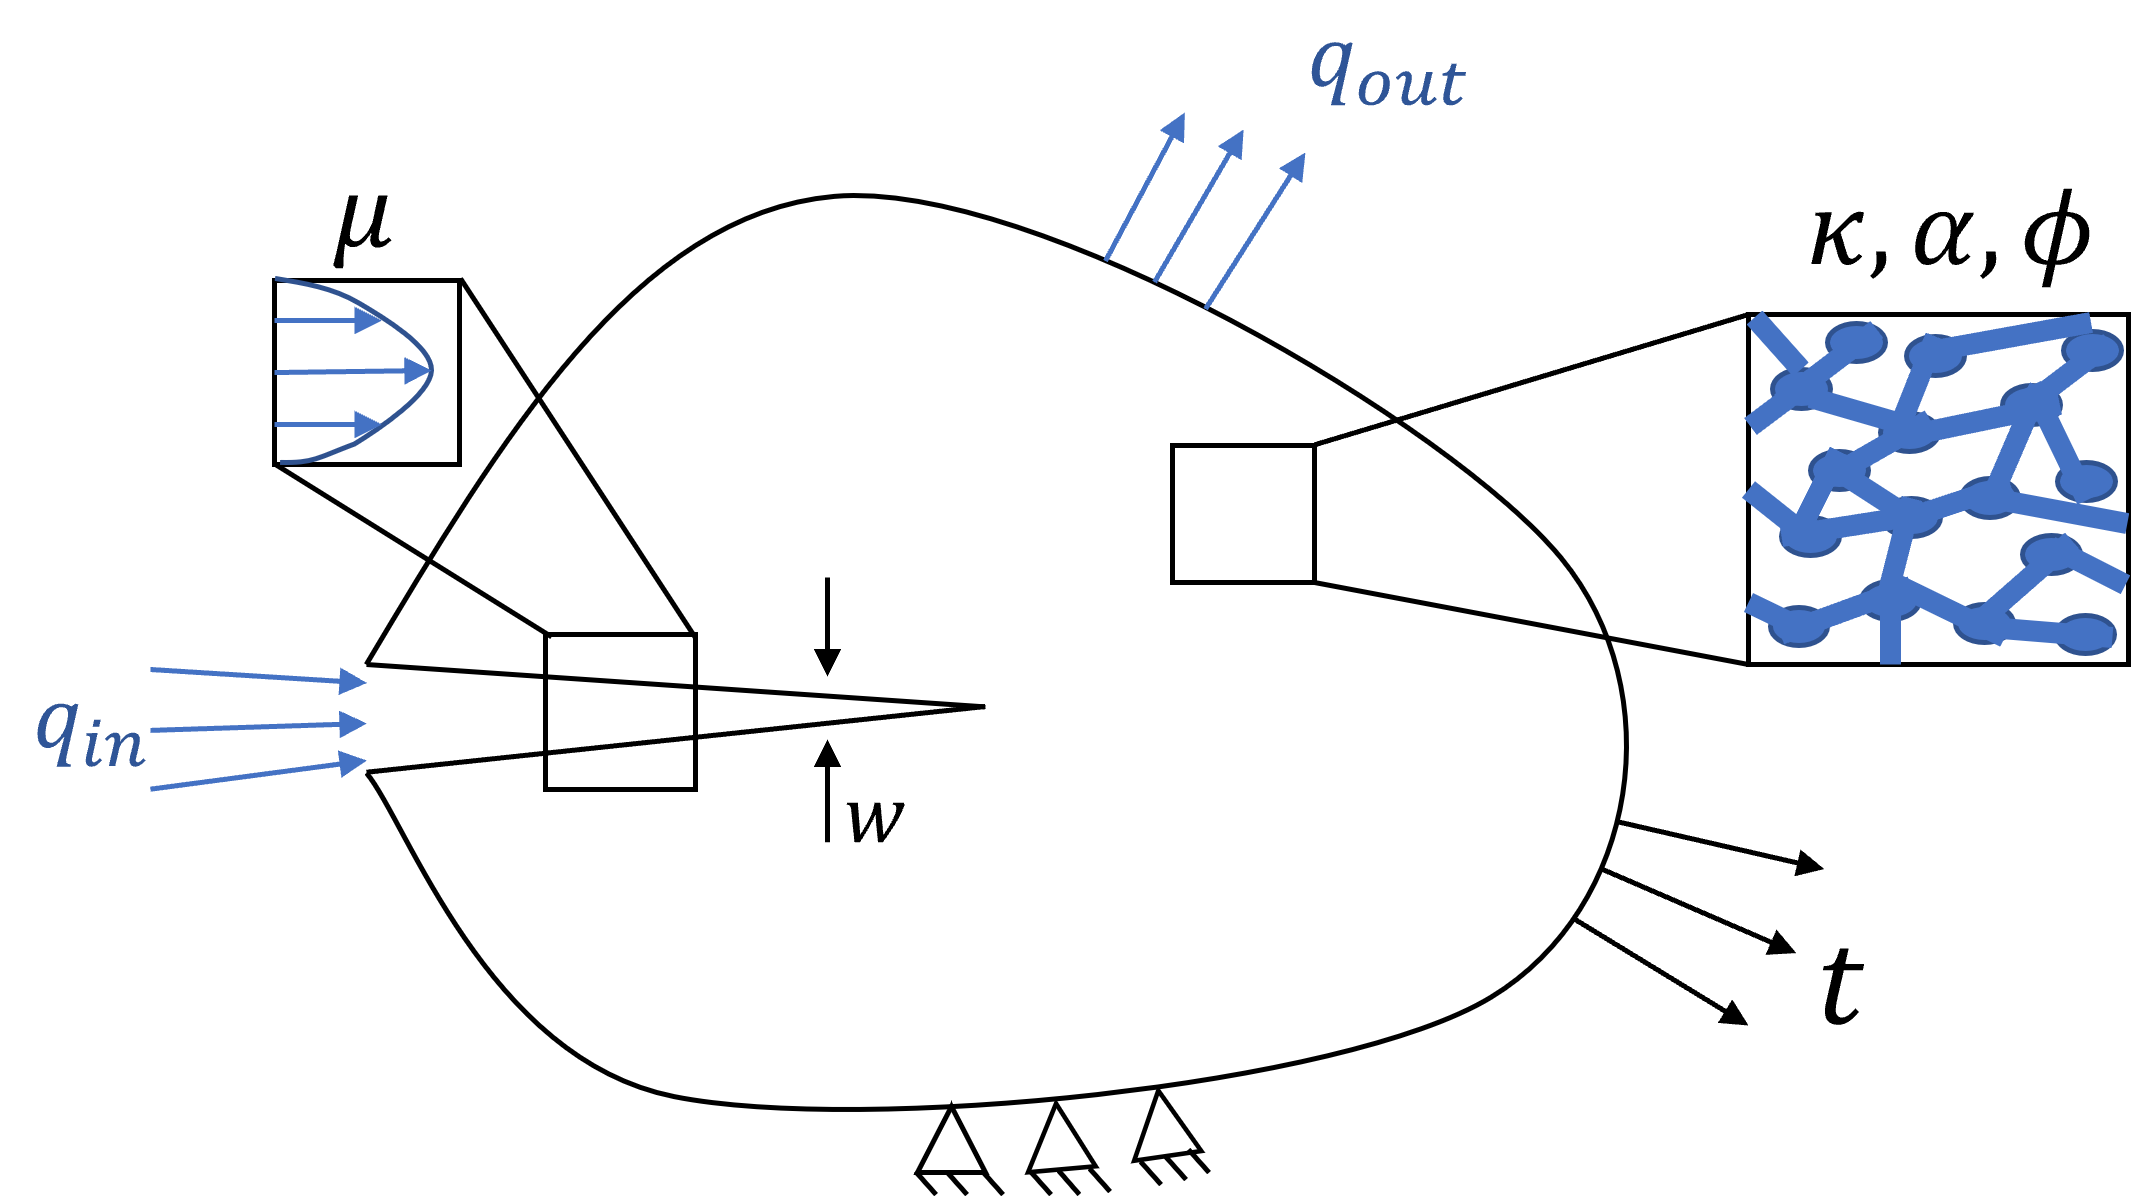
\includegraphics[width=15cm]{img/HF_potato_regular.png}
    \caption{Schematic of a poroelastic rock with a fracture, inspired by \cite{landis2016birs}.}
    \label{fig:potato_rock}
\end{figure}

We consider a model that couples flow and elastic deformation in a porous media with evolving fracture surfaces.  Consider the domain $\Omega$ consisting of a porous rock, that is fully saturated with a single-phase Newtonian fluid. The external boundary is composed of both traction $\partial \Omega_t$ and displacement $\partial \Omega_u$ surfaces, viz.\  $\partial \Omega = \partial \Omega_t \cup \partial \Omega_u$. 

The domain contains fractures $\Gamma$, as shown in Figure \ref{fig:potato_rock}.  For simplicity, we assume quasi-static conditions and small-strain kinematics.   Neglecting inertial effects, the balance of linear momentum reads
\begin{equation}\label{linear momentum balance}
    \nabla \cdot \boldsymbol\sigma + \textbf{b} = \boldsymbol 0\ \text{on } \Omega\setminus\Gamma,
\end{equation}
where $\boldsymbol\sigma$ denotes the total Cauchy stress and $\textbf{b}$ the body force. The mechanical boundary conditions are given by
\begin{equation}\label{traction bc}
    \boldsymbol \sigma \cdot \textbf{n} = \textbf{t} \text{ on } \partial \Omega_t,
\end{equation}
\begin{equation}\label{displacement bc}
    \textbf{u} = \overline{\textbf{u}} \text{ on } \partial \Omega_u,
\end{equation}

where $\textbf{n}$ denotes the normal direction at any point on $\partial\Omega$,  $\textbf{t}$ are the applied tractions, and $\overline{\textbf{u}}$ denotes the prescribed displacements.

Fluid flow within the cracks gives rise to pressure loads on the crack surfaces, translating into the boundary condition 
\begin{equation}\label{fracture boundary condition}
    \boldsymbol\sigma^+\cdot \textbf{n}_{\Gamma} = -\boldsymbol\sigma^-\cdot \textbf{n}_{\Gamma} = -p_f\textbf{n}_{\Gamma} \text{ on } \Gamma,
\end{equation}
where $p_f$ is the pressure inside the crack and $\textbf{n}_{\Gamma}$ is the normal vector to $\Gamma$ at any point.  In this work, we assume that fractures are open and neglect contact conditions on crack faces.  For additional considerations to account for closed fractures, see the model described in Cusini et al.\cite{cusini2021simulation}.

In terms of the fluid flow, the fluid velocity $\textbf{v}_m$ in the matrix is governed by the mass balance 
\begin{equation}\label{mass balance matrix}
    \dfrac{\partial(\rho \phi)}{\partial t} + \nabla \cdot (\rho \textbf{v}_m) = Q_m + Q_{mf}\ \text{on } \Omega\setminus\Gamma.
\end{equation}
where $\rho$ denotes the fluid density and $\phi$ is the porosity, and $Q_m$ is a prescribed source term in the matrix. The source term $Q_{mf}$ accounts for the exchange of fluid between the matrix and the fractures.
The boundary is partitioned into pressure $\partial \Omega_p$ and flux $\partial\Omega_q$ portions, such that $\partial \Omega = \partial \Omega_p \cup \partial \Omega_q$, and the following boundary conditions are applied,

\begin{equation}\label{flux bc}
    \rho \textbf{v}_m \cdot \textbf{n} = \textbf{q} \text{ on } \partial \Omega_q,
\end{equation}

\begin{equation}\label{pressure bc}
    p_m = \overline{p}_m \text{ on } \partial \Omega_p,
\end{equation}

where $p_m$ denotes the pore-pressure and  $\overline{p}_m$ is a prescribed pressure.

In a comparable manner, the fluid velocity $\textbf{v}_f$ within fractures is governed by the mass balance
\begin{equation}\label{mass balance fracture}
    \dfrac{\partial(\rho w)}{\partial t} + \nabla_{\Gamma} \cdot (\rho w \textbf{v}_f) = Q_f + Q_{fm}\ \text{on } \Gamma,
\end{equation}
where $w$ denotes the normal fracture aperture, $Q_f$ is a prescribed source term within the fracture, and $Q_{fm}$ accounts for the exchange of fluid between the fracture and the matrix\footnote{the flux interactions $Q_{fm}$ and $Q_{mf}$ are modeled as in classical well models, following \cite{hajibeygi2011hierarchical}. This ensures the balance of mass between the fractures and matrix $\int_V Q_{mf} dV = -\int_{\Gamma}Q_{fm}d\Gamma$.}. In the above, $\nabla_{\Gamma}$ indicates a gradient operator taken on the lower dimensional manifold  $\Gamma$. Boundary conditions similar to \eqref{flux bc} and \eqref{pressure bc} can also be applied.

Constitutive relationships are required to close the system and tie the stresses to the displacements $\textbf{u}$ and the fluid velocities to the pressures. In particular, we adopt the basic assumptions of Biot's theory of poroelasticity \cite{biot1941general}, Darcy's law for the flow in the matrix, and a lubrication theory approximation for the flow in fractures. This gives rise to the following set of constitutive relationships for the stress, porosity, and velocities:

\begin{equation}\label{biot law}
    \boldsymbol \sigma = \mathbb{C}:\boldsymbol\epsilon(\textbf{u}) - \alpha p_m \mathbb{I} \ \text{on } \Omega\setminus\Gamma,
\end{equation}

\begin{equation}\label{linear porosity}
    \dot{\phi} = \alpha \nabla \cdot \dot{\textbf{u}} + \dfrac{\dot{p_m}}{N} \ \text{on } \Omega\setminus\Gamma,
\end{equation}

\begin{equation}\label{darcy law}
    \textbf{v}_m = -\dfrac{\kappa}{\mu}\nabla p_m \ \text{on } \Omega\setminus\Gamma,
\end{equation}

\begin{equation}\label{cubic law}
    \textbf{v}_f = -\dfrac{w^2}{12\mu}\nabla_{\Gamma} p_f \ \text{on } \Gamma.
\end{equation}

In the above, $p_m$ is the pore-pressure, $\mathbb{C}$ is the fourth-order isotropic tensor of drained elastic moduli,  $\boldsymbol\epsilon(\textbf{u})$ is the mechanical strain, $\alpha$ is the Biot coefficient, and $\mathbb{I}$ is the second-order identity tensor. The temporal evolution of the porosity is governed by the rate of dilatation and time rate of change in the pore pressure, as modulated by the modulus $N$.  The fluid velocity in the matrix is related to the gradient of the pressure through the ratio of the intrinsic permeability $\kappa$ to the viscosity $\mu$.    

The fluid is assumed to be linearly compressible.  For both the fluid in the fractures and the matrix, this implies that the density is updated from its reference value $\rho_{ref}$ based on the change in pressure according to
\begin{equation}\label{poorly compressibility}
    \rho = \rho_{ref} \left(1 + \dfrac{p  - p_{ref}}{K_F}\right) \ \text{on } \Omega,
\end{equation}
where $p_{ref}$ denotes a reference value for the pressure, and $K_F$ is the fluid bulk modulus. 

Finally, the initial conditions for the displacements and pressures are given by

\begin{equation}\label{u_ic}
    \textbf{u}(\textbf{x},0) = \textbf{u}^0  \ \text{on } \Omega\setminus\Gamma,
\end{equation}

\begin{equation}\label{pm_ic}
    p_m(\textbf{x},0)= p^0_m  \ \text{on } \Omega\setminus\Gamma,
\end{equation}

\begin{equation}\label{pf_ic}
    p_f(\textbf{x},0) = p^0_f  \ \text{on } \Gamma.
\end{equation}

For a given crack geometry, the combination of equations \eqref{linear momentum balance}, \eqref{mass balance matrix} and \eqref{mass balance fracture}, with constitutive assumptions \eqref{biot law} - \eqref{poorly compressibility}, boundary conditions \eqref{traction bc}-\eqref{fracture boundary condition},\eqref{flux bc},\eqref{pressure bc} and initial conditions \eqref{u_ic}-\eqref{pf_ic} leads to a system of equations whose solution can be approximated by many different numerical methods.
What remains is a model to describe the evolution of the crack geometry.

In the context of standard sharp interface approaches for hydraulic fracture, the evolution of the crack geometry is typically governed by a set of criteria that dictate whether or not a crack front extends and, if so, in what orientation.  For crack extension, a standard approach is to adopt Griffith's criteria \cite{griffith1921vi}, which states that crack propagation should occur when the energy release rate $G$ reaches the critical value $G_c$ for the material, i.e.\ $G \le G_c$.   In terms of changes to orientation, several different criteria are typically employed, such as the maximum hoop stress criteria \cite{10.1115/1.3656897, williams1972fracture, finnie1973note} or the maximum energy release rate condition \cite{ewing1976further, cotterell1965brittle, hussain1974strain}. Examples of works from the hydraulic fracture field employing such criteria include \cite{he2018modeling, jang2020analysis, grossman2019algorithm}. 

Although such methods have seen some success in simulating the propagation of hydraulically-driven cracks, even in three dimensions \cite{gupta2014simulation, gupta2018coupled,shauer2022three}, they struggle as crack evolution becomes sufficiently complex.  By contrast, regularized methods have seen far more success in treating complex geometric evolution. In the next subsection, we present the governing equations for a phase-field method for fracture, a regularized approach for representing fractures and their evolution.  Phase-field for fracture models generally start from a single energetic postulate that generalizes Griffith's criteria, and which is able to describe the entire fracture propagation process.

\subsection{The phase-field method for fracture}
\label{sec:pfm-fracture}

The phase-field method for fracture started as an approximation \cite{bourdin2000numerical} to the variational approach for fracture by Francfort and Marigo \cite{francfort1998revisiting} for the quasi-static propagation of fracture in brittle materials. This model essentially states that a crack should evolve in a way that minimizes a total energy functional, among all admissible states, which are those that contain the current crack set (so that no healing is possible). For the method adopted in this work, we follow the work of Chukwudozie et al.\ \cite{chukwudozie2019variational} and associate the following total energy to a crack configuration $\Gamma$ in a poroelastic brittle solid $\Omega$:
% \begin{multline}\label{variational approach to fracture}
%     \mathcal{E}(\textbf{u}, p_m, p_f, \Gamma) = \int\limits_{\Omega \setminus \Gamma}W(\boldsymbol{\epsilon}(\textbf{u}), p_m)d\Omega - \int\limits_{\partial\Omega_N} \textbf{t} \cdot \textbf{u} ds
%     - \int\limits_{\Omega\setminus \Gamma} \textbf{b} \cdot \textbf{u} d\Omega \\
%     + \int\limits_{\Gamma}p_f \llbracket \textbf{u} \cdot \textbf{n}_{\Gamma} \rrbracket ds + G_c \mathcal{H}^{n-1}(\Gamma),
% \end{multline}
where the tractions applied to the boundary are denoted by $\textbf{t}$, the normal to the crack is denoted by $\textbf{n}_{\Gamma}$ and $\mathcal{H}^{n-1}(\Gamma)$ is the $n-1$ dimensional Hausdorff measure of $\Gamma$. 

The strain energy density $W(\boldsymbol{\epsilon}(\textbf{u}), p_m)$ is postulated as,

\begin{equation}
    W(\boldsymbol{\epsilon}(\textbf{u}), p_m) = \dfrac{1}{2}\left( \boldsymbol\epsilon(\textbf{u}) - \dfrac{\alpha}{nK} p_m\mathbb{I}\right) : \mathbb{C} : \left( \boldsymbol\epsilon(\textbf{u}) - \dfrac{\alpha}{nK} p_m\mathbb{I}\right),
\end{equation}

with $K$ denoting the bulk modulus and $n$ the system's dimension (2 or 3). The phase-field regularization, based on the Ambrosio-Tortorelli \cite{ambrosio1990approximation} functional is then performed by the introduction of the damage parameter $d$ and the regularization length $\ell$,

\begin{multline}\label{Poroelastic PF funcional}
    \mathcal{E}_{\ell}(\textbf{u},d,p_m,p_f) = \int\limits_{\Omega }\widetilde{W}(\boldsymbol{\epsilon}(\textbf{u}), p_m, d)d\Omega - \int\limits_{\partial\Omega_N}\textbf{t} \cdot \textbf{u} ds \\
    - \int\limits_{\Omega} \textbf{b} \cdot \textbf{u} d\Omega
    + \int\limits_{\Omega}p_f \textbf{u} \cdot \nabla d d\Omega 
    + \dfrac{G_c}{c_0}\int\limits_{\Omega }\left(\dfrac{\zeta(d)}{\ell} + \ell\nabla d\cdot\nabla d  \right)d\Omega,
\end{multline}

where the function $\zeta(d)$ is the local dissipation function, which is usually taken as $\zeta(d) = d$ or $d^2$. The constant $c_0$ is given by $c_0 = 4\int_0^1 \sqrt{\zeta(z)}dz$ and the regularized strain energy is defined by,

\begin{equation}\label{damaged strain energy}
    \widetilde{W}(\boldsymbol{\epsilon}(\textbf{u}), p_m, d) = \dfrac{1}{2}\left( (1-d)\boldsymbol\epsilon(\textbf{u}) - \dfrac{\alpha}{nK} p_m\mathbb{I}\right) : \mathbb{C} : \left( (1-d)\boldsymbol\epsilon(\textbf{u}) - \dfrac{\alpha}{nK} p_m\mathbb{I}\right),
\end{equation}

which is consistent with an assumption of damage arising in the sub pore scale \cite{chukwudozie2019variational}. Finally, our regularized crack evolution problem is then stated as a minimization principle for the functional $\mathcal{E}_{\ell}(\textbf{u},d,p_m,p_f)$, with respect to the variables $\textbf{u}$ and $d$, with the added condition that the damage process is irreversible and that the damage variable $d$ is bounded between the values of zero (undamaged state) and unity (fully broken state):
\begin{equation}\label{variational formulation of phase-field}
    \textbf{u}, d = \underset{\textbf{u},d}{{\operatorname{argmin}}} \ \mathcal{E}_{\ell}(\textbf{u},d,p_m,p_f)\ \text{,\ \   subject to } \dot{d} \ge 0, \text{ and } 0 \le d \le 1. 
\end{equation}

The following set of evolution equations can then be derived from the Karush–Kuhn–Tucker (KKT) \cite{karush1939minima, kuhn1951nonlinear} conditions:

\begin{equation}\label{basic u problem}
    \nabla \cdot \left( (1-d)^2\ \mathbb{C}:\boldsymbol\epsilon(\textbf{u}) -(1-d)\alpha p_m \mathbb{I}\right) + \textbf{b} = p_f\nabla d, 
\end{equation}

\begin{equation}\label{damage equation ch3}
    S_d \coloneqq  \dfrac{2G_c\ell}{c_0}\Delta d - \dfrac{G_c}{c_0\ell}\zeta'(d)-g'(d)W(\boldsymbol{\epsilon}(\boldsymbol{\textbf{u}}),0) + \alpha p_m\nabla \cdot \textbf{u} + \nabla \cdot (p_f\textbf{u}) \le 0,
\end{equation}

\begin{equation}
    \dot{d} \ge 0,
\end{equation}

\begin{equation}
   0 \le d \le 1,
\end{equation}

\begin{equation}
    S_d\dot{d} = 0,
    \label{eq:ddot-strong}
\end{equation}

with boundary conditions, $\boldsymbol\sigma \cdot \textbf{n} = \textbf{t}$ on $\partial \Omega_N$ and $(2G_c\ell\nabla d +c_0p_f\textbf{u})\cdot \textbf{n} \ge 0$ on $\partial \Omega$. The damaged stress is defined as $\boldsymbol\sigma = (1-d)^2\ \mathbb{C}:\boldsymbol\epsilon(\textbf{u}) -(1-d)\alpha p_m \mathbb{I}$.

In some cases, it is useful to decompose the energy \eqref{damaged strain energy} into positive and negative parts, in order to provide asymmetry between tension and compression states. In most problems studied in this Chapter, we found this decomposition to be important, and, unless otherwise mentioned, the spectral decomposition introduced in Miehe et al.~\cite{miehe2010phase} is used. With this decomposition, the equations for the macro-scale force balance \eqref{basic u problem} and the micro-force balance \eqref{damage equation ch3} are modified as

\begin{equation}\label{basic u problem spectral}\tag{3.22a}
    \nabla \cdot \left( (1-d)^2\ \mathbb{C}:\boldsymbol\epsilon^+(\textbf{u}) + \mathbb{C}:\boldsymbol\epsilon^-(\textbf{u})-(1-d)\alpha p_m \mathbb{I}\right) + \textbf{b} = p_f\nabla d, 
\end{equation}

\begin{equation}\label{damage equation spectral}\tag{3.23a}
    S_d \coloneqq  \dfrac{2G_c\ell}{c_0}\Delta d - \dfrac{G_c}{c_0\ell}\zeta'(d)-g'(d)W(\boldsymbol{\epsilon^+}(\boldsymbol{\textbf{u}}),0) - \alpha p_m\nabla \cdot \textbf{u} + \nabla \cdot (p_f\textbf{u}) \le 0,
\end{equation}

and the damaged stress becomes $\boldsymbol\sigma = (1-d)^2\ \mathbb{C}:\boldsymbol\epsilon^+(\textbf{u}) + \mathbb{C}:\boldsymbol\epsilon^-(\textbf{u})-(1-d)\alpha p_m \mathbb{I}$. In the above, $\boldsymbol\epsilon^+$ and $\boldsymbol\epsilon^-$ denote the positive and negative parts of the strain tensor as described in \cite{miehe2010phase}. 

Finally, to close this section, we note that the extent to which the solution to \eqref{variational formulation of phase-field} approaches a particular sharp model in hydraulic fracture in the limit as the regularization length $\ell\rightarrow 0$ has yet to be established.  Nevertheless, the particular phase-field model adopted here contains all of the requisite components to allow for a proof of concept of the multi-resolution approach.  




